\documentclass[11pt,a4paper]{article}

\usepackage{url,,}
\usepackage{graphicx}
\usepackage{hyperref}
\usepackage{amsfonts}
\usepackage{amssymb}
\usepackage{amsmath}
\usepackage{amsfonts}
\usepackage{amssymb}
\usepackage{amsmath}
\usepackage{multirow}
\usepackage{listings}
\usepackage{fullpage}
\usepackage{fancyhdr,a4wide}
\usepackage{makeidx}
\usepackage{placeins}
\usepackage[procnames,noindent]{lgrind}

\lstset{ %
language=VHDL,                % choose the language of the code
basicstyle=\footnotesize,       % the size of the fonts that are used for the code
showstringspaces=false,         % underline spaces within strings
%numbers=left,                   % where to put the line-numbers
%numberstyle=\footnotesize,      % the size of the fonts that are used for the line-numbers
%stepnumber=1,                   % the step between two line-numbers. If it's 1 each line will be numbered
%numbersep=5pt,                  % how far the line-numbers are from the code
%backgroundcolor=\color{white},  % choose the background color. You must add \usepackage{color}
showspaces=false,               % show spaces within strings adding particular underscores
showtabs=false,                 % show tabs within strings adding particular underscores
escapeinside={\%*}{*)}          % if you want to add a comment within your code
}

\begin{document}	

\begin{titlepage}

\thispagestyle{fancy}
\lhead{}
\chead{
\large{\textit{
Informatics and Mathematical Modelling\\
Technical University of Denmark}}}
\rhead{}
\rule{0pt}{50pt}
\vspace{3cm}

\begin{center}

 	\huge{\textbf{02207 : Advanced Digital Design Techniques}}\\
 	\vspace{1cm}
 	\huge{Design for Low Power by Reducing Switching Activity}\\
 	\vspace{1cm}
 	\huge{\textit{LAB 2}}\\
 	\vspace{1cm}
 	\huge{Group \textit{dt07}}\\
\end{center}

\vspace{4cm}

\begin{flushright}
	\LARGE{Markku Eerola (s053739)}\\
	\vspace{0.3cm}
	\LARGE{Rajesh Bachani (s061332)}\\
	\vspace{0.3cm}
	\LARGE{Josep Renard (s071158)}\\
\end{flushright}
\cfoot{\today}
\end{titlepage}

%\begin{abstract}
%\centering
%Abstract to be created.
%\end{abstract}

%-----------------------------------------------------------
\newpage 
\tableofcontents

\newpage 
\section{Introduction}

The purpose of this exercise was to estimate the power dissipation in a digital circuit due to the switching activity in the cells. Power is dissipated in a digital circuit, dynamically, in two ways; one, the power that is spent in charging or discharging the capacitance load connected to the output of the cell, and two, the power dissipated inside the cell due to short circuit currents and the internal capacitance charging or discharging. This holds for combinational cells. For sequential cells, there is extra power spent at every clock cycle, even if the output of the cell does not change. This is because there is some reaction to every clock cycle in sequential cells, which would take some power. 

Static power in digital circuits is due to the internal leakage currents in CMOS. Though, in this exercise, we are particularly interested in analyzing the dynamic power dissipation.

We estimate the dynamic power in a serial to parallel converter. The converter takes in 8 bits (one byte) in every clock cycle, and gives out 32 bits (4 bytes) after every 4 clock cycles. The input byte at the first clock cycle is the most significant byte in the output, whereas the input byte in the fourth clock cycle is the lowest significant byte. The converter, thus, waits for four clock cycles to produce an output. We refer to the register holding the most significant byte in the output as the most significant register, and that holding the least significant byte as the least significant register.

The report is organized as follows. In section \ref{section:designs}, we discuss three designs for a serial to parallel converter. In section \ref{section:simulation}, we simulate the VHDL code for the designs using Modelsim, and verify that all the designs are working correctly. Section \ref{section:power} contains the power results obtained from the synthesis of the VHDL using Design Vision, and Synopsys VSS for annotating the switching activity in a given time period. In this section, we discuss and justify the results obtained. Later, in section \ref{section:impl}, the VHDL is provided, alongwith the power reports from Design Vision. 

\subsection{Authors by Section}
\begin{itemize}
\item \textit{Rajesh Bachani} VHDL code for Design A, Design B and Design C, and simulation of the designs in Modelsim.
\item \textit{Josep Renard} Synthesis of the designs for power reports, using Synopsys VSS and Design Vision.
\item \textit{Markku Eerola} Discussion and Analysis of the power reports.
\end{itemize}

\newpage
\section{Designs for Serial to Parallel Conversion}
\label{section:designs}
In this section, we give an overview of the three designs for serial to parallel conversion, which are evaluated for their power consumption in this exercise.

\subsection{Design A: Shift Register}

\begin{figure}[htp]
\centering
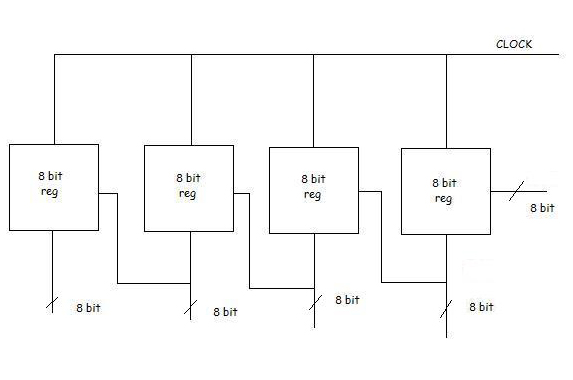
\includegraphics[width = 3.5in]{./images/shiftregister.jpg}
\caption{Converter using a 8-bit Shift Register}
\label{figure:sr}
\end{figure}

As we can see in figure \ref{figure:sr}, the input data flows continuously through the registers. On every rising clock edge each of the 8-bit registers takes on a new state. The least significant register takes its state from the input to the converter block and all the other registers take their states from the outputs of the adjacent less significant register. All components of this block are driven with the same clock signal, which ensures that the 8-bit registers change their state at the same time as the clock signal event. 


\subsection{Design B: Register with Enable}

\begin{figure}[htp]
\centering
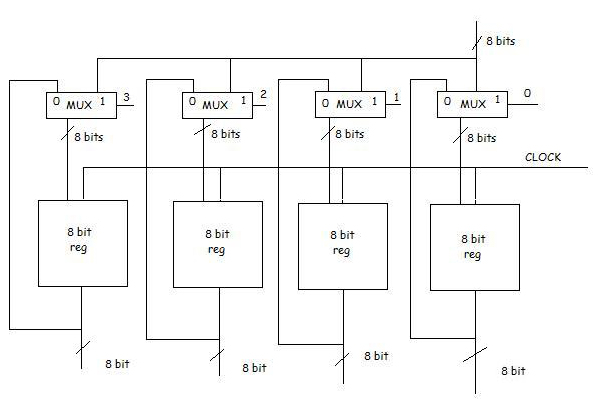
\includegraphics[width = 3.5in]{./images/shiftregisterenable.jpg}
\caption{Converter using 8-bit Registers with Enable}
\label{figure:sre}
\end{figure}

In figure \ref{figure:sre} we see another design for a serial to parallel converter. In this design we use multiplexers to control when the 8-bit registers should take on a new state. The multiplexers take in two inputs, one from the output of the 8-bit register connected with that multiplexer, and one from the input to the converter block, which is Qk. When the enable signal to a multiplexer is SET, it lets through Qk, whereas, in the other case, it lets through the data from the 8-bit register's output, thus retaining the register's previous state. The enable signal to the four multiplexers is changed in a sequence, with the multiplexer 3 getting the enable first, and the multiplexer 0 getting the enable last. This way, the value of Qk in the first clock cycle is transferred to the most significant register, while Qk in the fourth clock cycle is transferred to the least significant register.
\

\subsection{Design C: Register with Clock-Gating}

\begin{figure}[htp]
\centering
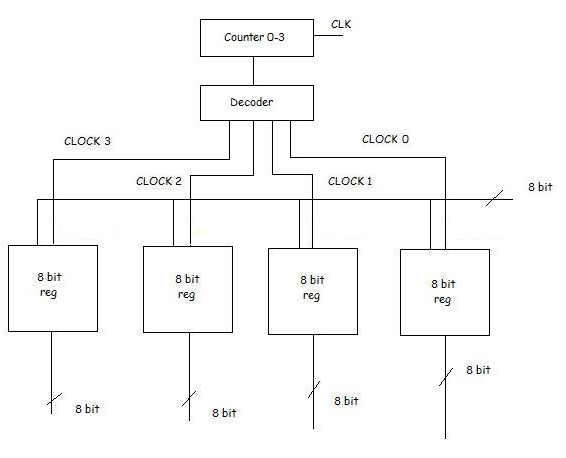
\includegraphics[width = 3.5in]{./images/shiftregistergated.jpg}
\caption{Converter using 8-bit Registers with Clock Gating}
\label{figure:srg}
\end{figure}

In figure \ref{figure:srg} we see the third design for a serial to parallel converter we used in the exercise. In this design we restirct the amount of register state changes by not driving the 8-bit registers with the clock directly but instead using a 2-bit counter and a 2:4 decoder to give a rising clock edge only to one of the four 8-bit register's at a time. In this design the 8-bit registers operate only when they change their state once every fourth clock cycle. This means that they consume much less power. Of course the logic for dividing the clock consumes power as well, but we expect that the power savings which are gained by reducing the operation of the 8-bit registers outweighs this, since we're not only restricting the number of state changes but we're also completely removing the power consumption for 'idle' operations.


\newpage
\section{Simulation of the designs with Modelsim}
\label{section:simulation}
All the three designs are simulated with Modelsim, to verify the functionality.
 
The following two screenshots demonstrate the working of implementation for Design A. The first screenshot is taken at 33ns while the second is taken at 43ns. It can be seen that in the new clock cycle, the 8 bit registers have rippled their values to the more significant register, and the value of Qk for that clock cycle is fed into the least significant register. The most significant register looses its old value.

\begin{figure}[htp]
\centering
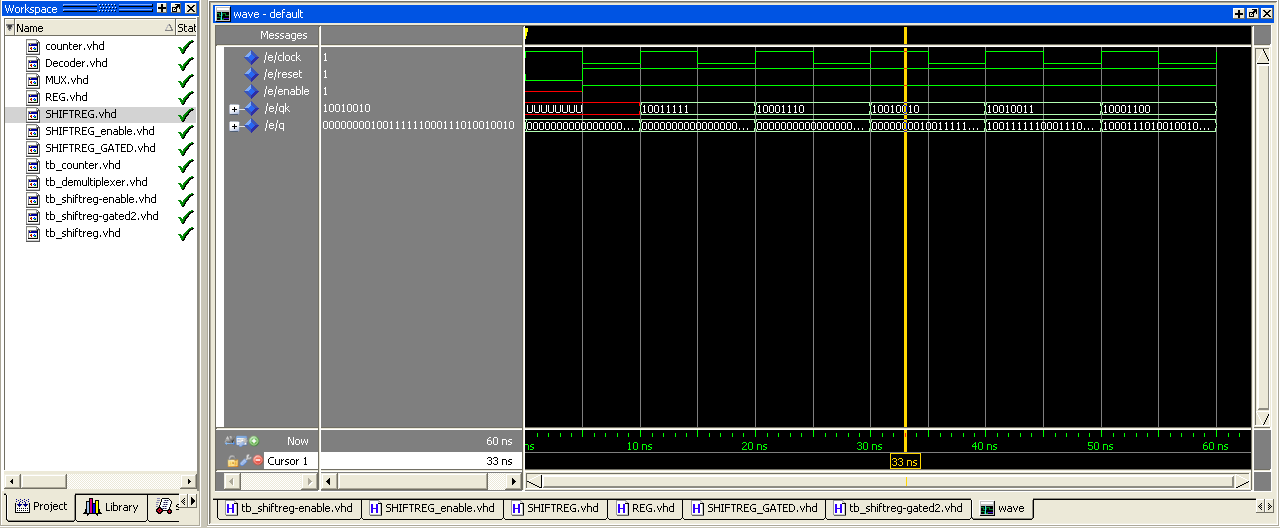
\includegraphics[length = 4in,width = 6.5in]{./images/simsr1.png}
\caption{Simulation screenshot for Design A at 33ns}
\end{figure}

\begin{figure}[htp]
\centering
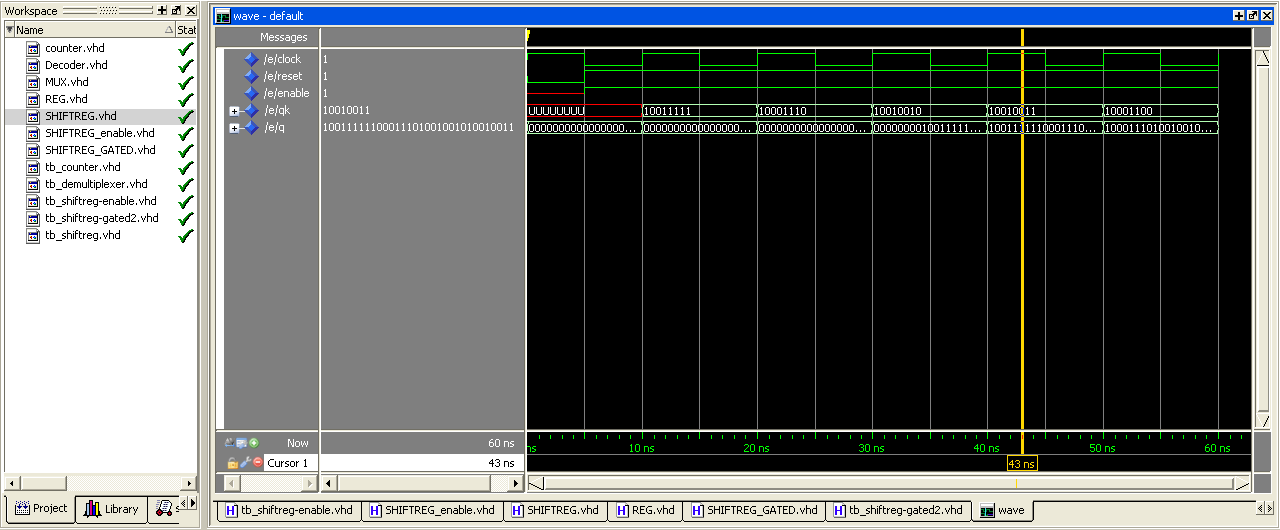
\includegraphics[length = 4in,width = 6.5in]{./images/simsr2.png}
\caption{Simulation screenshot for Design A at 43ns}
\end{figure}

\newpage
The following screenshots are from the simulation of Design B. In the first instance, at 14ns on the timeline, we have some value at Qk, but it has not been transferred in any way to the output Q. Then, at 24ns, the value of Qk in the previous clock cycle is loaded into the most significant register. Further on, at 33ns, the value of Qk in the previous clock cycle is loaded into the second most significant register. This repeats for four clock cycles, after which the most significant register is again loaded.

\begin{figure}[htp]
\centering
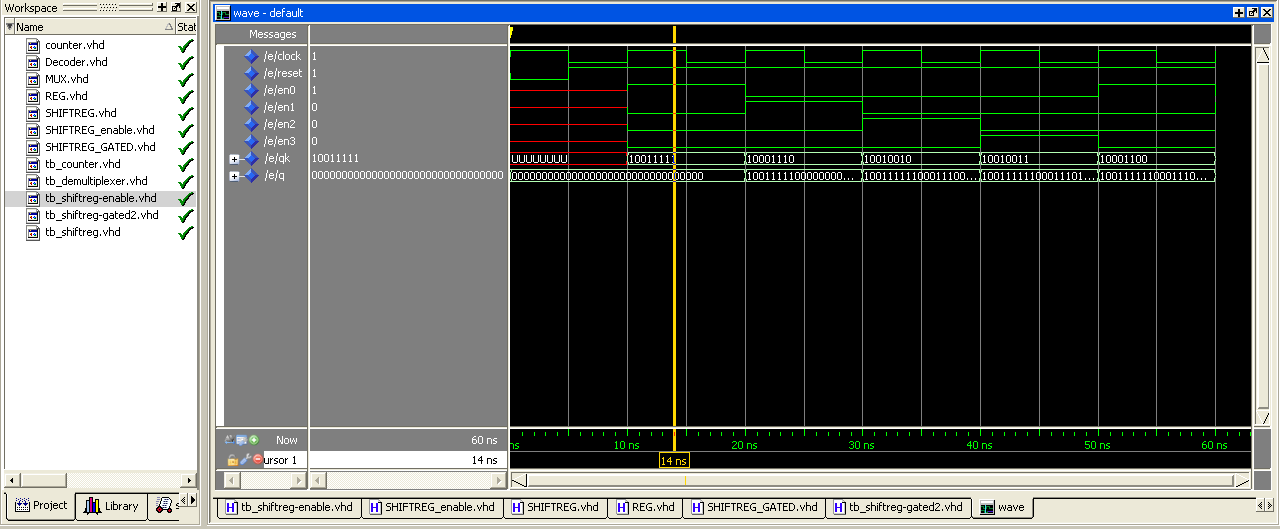
\includegraphics[length = 4in,width = 6.5in]{./images/simsre1.png}
\caption{Simulation screenshot for Design B at 14ns}
\end{figure}

\begin{figure}[htp]
\centering
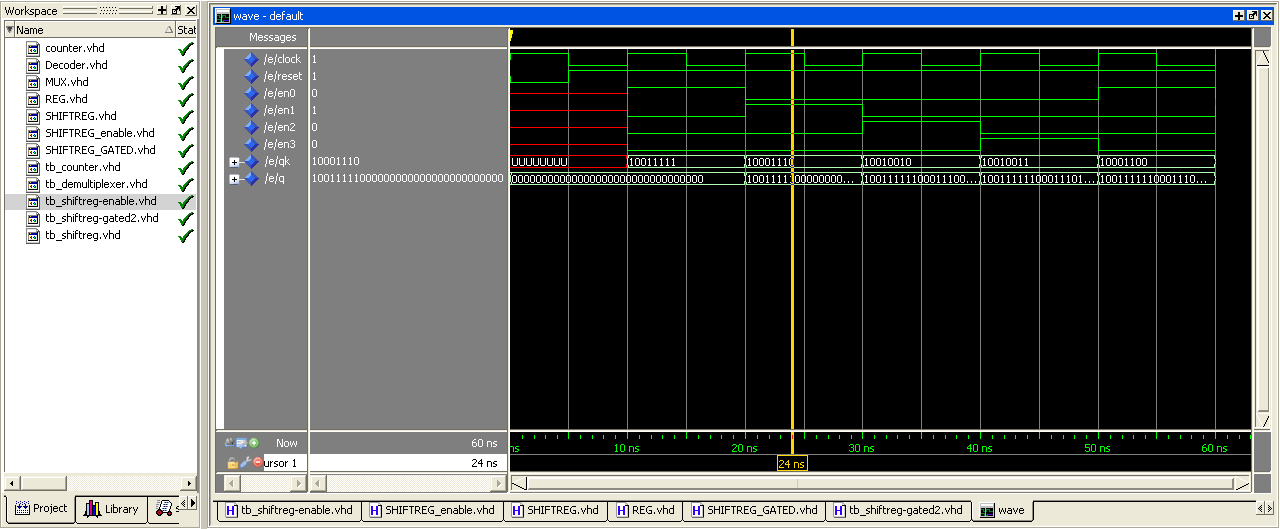
\includegraphics[length = 4in,width = 6.5in]{./images/simsre2.png}
\caption{Simulation screenshot for Design B at 24ns}
\end{figure}

\begin{figure}[htp]
\centering
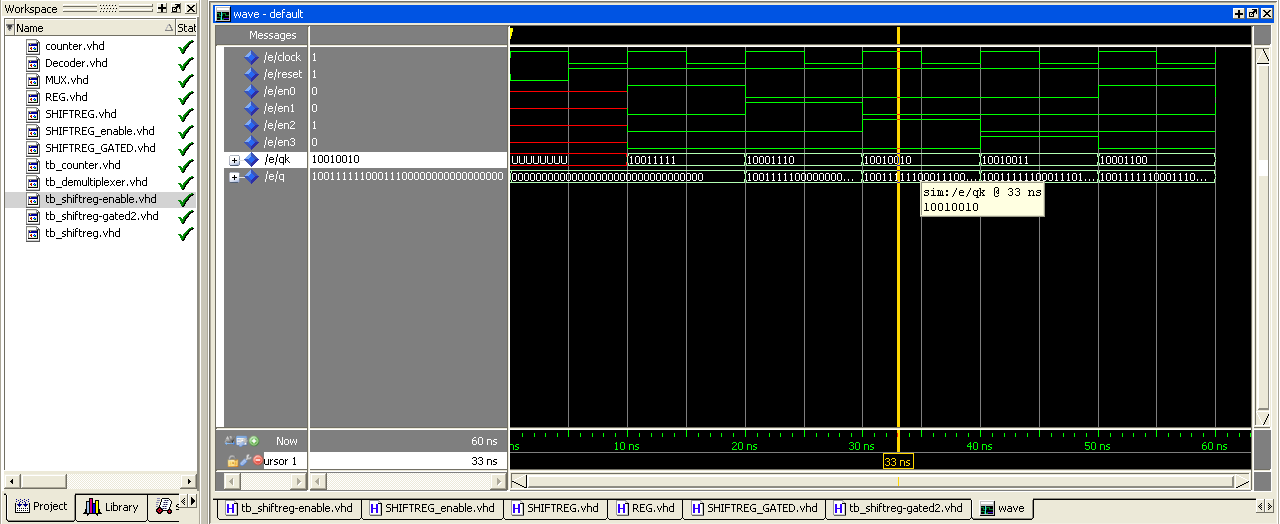
\includegraphics[length = 4in,width = 6.5in]{./images/simsre3.png}
\caption{Simulation screenshot for Design B at 33ns}
\end{figure}

\newpage
Then, for Design C, we have the following screenshots. As we can see, the values of Qk are transferred to different registers every clock cycle. This is practically the same functionality as Design B. The only difference though is that in Design C, Qk is transferred in the same clock cycle, while in Design B, it happens one clock cycle later. Ofcourse, the internal working of the two designs are completely different, which has already been discussed in section \ref{section:designs}

\begin{figure}[htp]
\centering
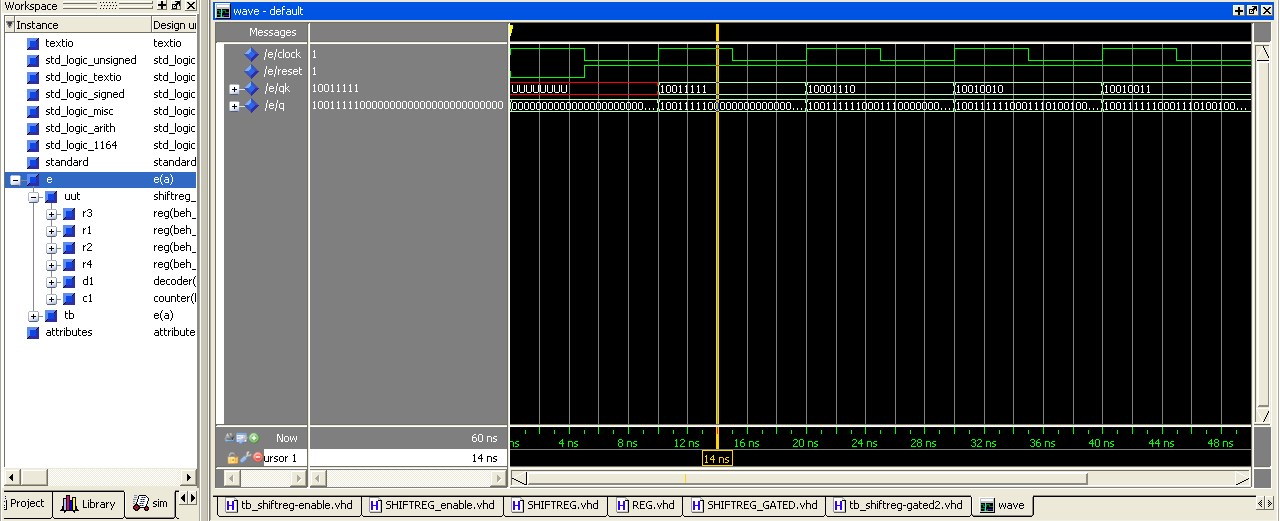
\includegraphics[length = 4in,width = 6.5in]{./images/simsrg1.png}
\caption{Simulation screenshot for Design C at 14ns}
\end{figure}

\begin{figure}[htp]
\centering
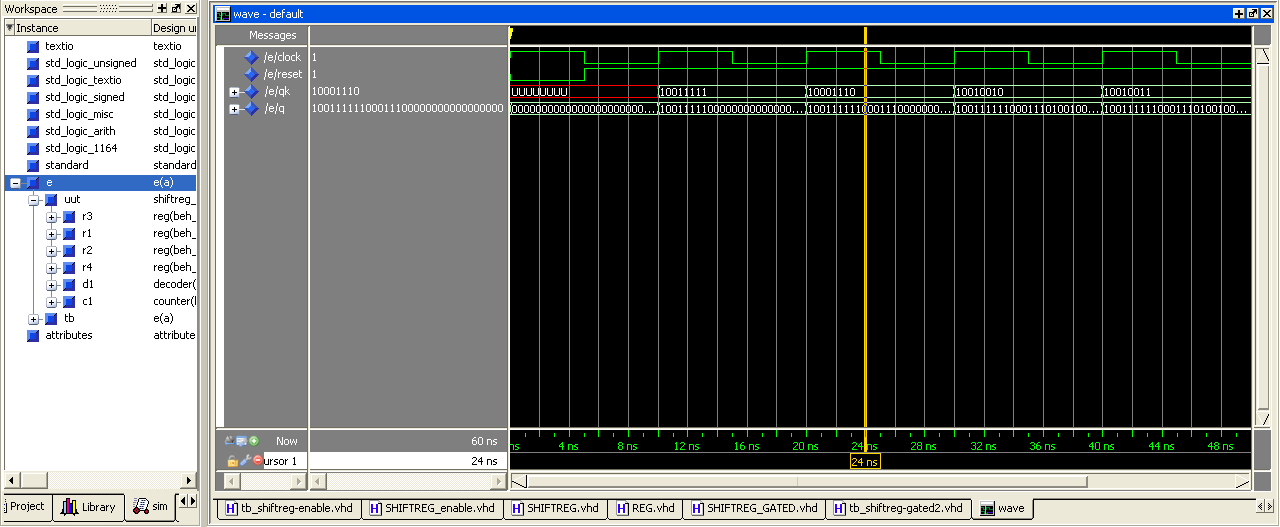
\includegraphics[length = 4in,width = 6.5in]{./images/simsrg2.png}
\caption{Simulation screenshot for Design C at 24ns}
\end{figure}

\newpage
\section{Power Reports and Discussion}
\label{section:power}

In this section we discuss the results obtained from the power-aware synthesis of the three designs. The Synopsys VSS Simulator is used to annotate the switching activity, based on a testbench for each design. This switching activity is used by Design Vision to estimate the total dynamic power consumption for the design. We have synthesized the designs for clock time periods of 2ns and 10ns and got the same results for all three designs for both clock periods. The power reports obtained from the synthesis are presented in section \ref{section:impl}. For a short recap the results can be seen in table \ref{table:power}:

\begin{table}[htbp]
\begin{center}
\begin{tabular}{|l|l|l|}
\hline
\textbf{}	& \textbf{Total Dynamic Power}		& \textbf{Cell Leakage Power}\\ \hline
Design A &	55.2 uW				& 773.7 nW \\ \hline
Design B &	47 uW					& 800.5 nW \\ \hline
Design C &  32.6 uW				& 835.0 nW \\ \hline
\end{tabular}
\end{center}
\caption{Overview of Results from Power Reports}
\label{table:power}
\end{table}

According to the results design A has the highest dynamic power consumption while design C has the least. We expected as much from design C, but from what we had learned on the lectures we had expected that design B would have consumed more power than design A. The static power consumption which comes from the internal leakage currents, is considerably lower than the dynamic power consumption in all of the designs. This is because static power consumption just depends on the number of cells in the design and does not depend on the switching activity. In the following analysis, we will only consider the dynamic power consumption and from now on when we use the word power we refer to the dynamic power.

In Design A the 8-bit registers change their state on each clock cycle. The input Qk is transferred from one register to the adjacent more significant register, every clock cycle, until it reaches the most significant register. This is the reason why the design is much consuming in terms of power: in every clock cycle, there is a switching activity in all the output bits of the four registers. Since switching accounts for a lot of power, for a given time line of the simulation, we have high levels of power consumption. 

Design B is more efficient than Design A from what is seen in the dynamic power consumption. Switching in Design B is controlled by the enable signals, which indicate which register should be loaded with Qk in the next clock event. If the enable signal is SET, the register is loaded with Qk, otherwise the output of the register is reloaded back into the register. Where the former case consumes a lot of dynamic power since the output bits are changed, the latter consumes less dynamic power which is due to internal response to the clock signal. So, since the registers still consume internal power on each clock cycle and since the multiplexers and the logic generating their enabling signals, both add to the overall power consumption, Design B should be less efficient than Design A for the overall power consumption. This is backed up by the lecture notes: the ratio of power dissipated in Design A to that in Design B is 1:1.19, which indicates that Design B should consume more power. We believe that the reason why our results differed from this is that the logic that generated the enabling signals was within the testbench instead of the converter and thus its power dissipation was not considered in the power analysis.

Lets consider Design C now. It is quite clear that this design is most efficient among the three. This design is based on clock-gating, which means that the original clock signal is not sent directly to the registers, but sent only when the register should be loaded with a new value. So, if there is a clock signal, the register funtions normally, and power is dissipated both internally and for charging/discharging the load (if the output changes). So, 75\% of the time the clock would be cut off completely, thus saving at least the internal power dissipation due to clock cycles. In Design B, even if the enable for a register was RESET, which meant that the register output would not change, there was still internal power dissipation in the cell for every clock cycle. This is avoided in Design C since the registers do not get clock signals except when they are supposed to change their state.

We see that the attempt to reduce power disspation has been successful, without affecting the functionality of the circuit. With the reduction in power consumption come some costs, in the form of extra area and time delay. The extra logic in designs B and C use up more area and some delay is also added to the critical path. It should also be noted, that in Design C the rising clock events for the 8-bit registers come a bit later than the event at the actual clock signal, which is referred to as skew. This means that the clock period must not be shorter than the delay or the circuit will not work properly.


\newpage
\section{Implementation and Power Reports}
\label{section:impl}

\lstinputlisting[frame=trbl, caption={SHIFTREG.vhd}]{../code/SHIFTREG.vhd}
\newpage
\lstinputlisting[frame=trbl,caption={SHIFTREG\_ENABLE.vhd}]{../code/SHIFTREG_ENABLE.vhd}
\newpage
\lstinputlisting[frame=trbl,caption={SHIFTREG\_GATED.vhd}]{../code/SHIFTREG_GATED.vhd}
\newpage
\lstinputlisting[frame=trbl,caption={REG.vhd}]{../code/REG.vhd}
\lstinputlisting[frame=trbl,caption={MUX.vhd}]{../code/MUX.vhd}
\newpage
\lstinputlisting[frame=trbl,caption={COUNTER.vhd}]{../code/counter.vhd}
\lstinputlisting[frame=trbl,caption={DECODER.vhd}]{../code/DECODER.vhd}
\newpage
\lstinputlisting[frame=trbl, caption={Power Report Design A}]{../code/power_report1.txt}
\newpage
\lstinputlisting[frame=trbl, caption={Power Report Design B}]{../code/power_report2.txt}
\newpage
\lstinputlisting[frame=trbl, , caption={Power Report Design C}]{../code/power_report3.txt}
\end{document}